\documentclass[11pt,a4paper]{article}

\usepackage[margin=1in]{geometry}
\usepackage{amsmath,amssymb,amsfonts,bm}
\usepackage{booktabs}
\usepackage{graphicx}
\usepackage{subcaption}
\usepackage{float}
\usepackage{microtype}
\usepackage{xcolor}
\usepackage{hyperref}
\usepackage{cleveref}
\usepackage{enumitem}
\usepackage{tikz}
\usetikzlibrary{arrows.meta,backgrounds,fit,positioning}

\hypersetup{
  colorlinks=true,
  linkcolor=blue!50!black,
  citecolor=blue!50!black,
  urlcolor=blue!60!black
}

\newcommand{\R}{\mathbb{R}}
\newcommand{\Ghat}{\widehat{G}_{\theta}}
\newcommand{\uhat}{\widehat{u}_{\theta}}
\newcommand{\norm}[1]{\left\lVert #1\right\rVert}

\title{Learning a Low-Rank Green's Operator for the Two-Dimensional Poisson Equation with Physics-Informed Neural Networks}
\author{Zhao, Zhan-Li\\
\texttt{chao4011@gmail.com}}
\date{July 2026}

\begin{document}
\maketitle

\begin{abstract}
We present a physics-informed method for learning the Green's operator of the two-dimensional Poisson equation on a square domain. Rather than training a separate neural network for every forcing term, the proposed model approximates the Green's function and maps a family of right-hand sides to their corresponding solutions through numerical quadrature. To reduce the cost of representing the four-dimensional kernel $G(x,y,s,t)$, two independent neural networks encode the evaluation coordinates $(x,y)$ and source coordinates $(s,t)$. Their outputs are combined through a rank-$R$ inner product, yielding a separable approximation of the Green's function. Random Fourier features improve the representation of oscillatory spatial dependence, while Gauss--Lobatto--Legendre nodes, quadrature weights, and spectral differentiation matrices provide the numerical discretization. Training data are generated from Gaussian random Fourier fields for which both the solution and its Laplacian are known analytically. The loss combines solution reconstruction with a discrete Poisson residual. We compare the rank-50 factorized model (Plan A) with a direct four-input model (Plan B) on an unseen mixed-frequency solution and a non-Fourier polynomial solution. The two plans attain relative $L^2$ errors of $6.53\times10^{-1}$ and $5.73\times10^{-1}$, respectively, on the mixed-frequency test, and $4.79\times10^{-2}$ and $4.70\times10^{-2}$ on the polynomial test. Their maximum nodal errors are $2.72\times10^{-2}$ for Plan A and $1.96\times10^{-2}$ for Plan B in both tests. The results show accurate transfer to a smooth non-Fourier field but limited extrapolation beyond the frequency range represented during training.
\end{abstract}

\noindent\textbf{Keywords:} Poisson equation, Green's function, physics-informed neural network, neural operator, low-rank approximation, spectral collocation

\section{Introduction}

The Poisson equation is a fundamental elliptic partial differential equation (PDE) that appears in electrostatics, gravitation, diffusion, pressure projection, and numerous inverse problems. Classical finite-difference, finite-element, and spectral methods provide accurate solutions, but a new linear system generally has to be solved whenever the forcing term changes. This repeated-solve setting motivates operator-learning approaches that approximate the entire mapping from a forcing function to its solution.

Physics-informed neural networks (PINNs) incorporate differential equations into the training objective and can solve PDEs without a conventional labeled data set \cite{raissi2019pinn}. Neural operators extend this idea by learning mappings between function spaces rather than a single solution \cite{lu2021deeponet,li2021fno}. In the present work, the operator is represented through a learned Green's function. For a linear elliptic problem, the Green's function contains the response of the system to a point source and can therefore be reused for arbitrary admissible forcing terms.

A direct neural representation of $G(x,y,s,t)$ takes a four-dimensional input. On a tensor-product grid with $n$ points per coordinate, explicitly evaluating the kernel requires $n^4$ values. We address the expensive neural evaluation by introducing a low-rank separable form,
\begin{equation}
  \Ghat(x,y,s,t)=\sum_{r=1}^{R}\phi_{\theta,r}(x,y)\psi_{\theta,r}(s,t),
  \label{eq:lowrank}
\end{equation}
where two neural networks learn the response-side and source-side features. This construction resembles separation of variables and the branch--trunk factorization used by DeepONet \cite{lu2021deeponet}.

The main contributions of this implementation are:
\begin{enumerate}[leftmargin=2em]
  \item a low-rank neural parameterization of a four-dimensional Green's kernel using two two-dimensional networks;
  \item a training procedure based on random Fourier solution fields with analytically available forcing terms;
  \item a physics-informed objective that combines operator reconstruction and a spectral discrete PDE residual; and
  \item an implementation based on Gauss--Lobatto--Legendre (GLL) quadrature and differentiation, together with out-of-distribution tests on mixed-frequency and non-Fourier solutions.
\end{enumerate}

\section{Problem Formulation}

Let $\Omega=[-1,1]^2$. We consider the homogeneous Dirichlet problem
\begin{align}
  \Delta u(x,y) &= f(x,y), && (x,y)\in\Omega, \label{eq:poisson}\\
  u(x,y) &= 0, && (x,y)\in\partial\Omega. \label{eq:bc}
\end{align}
The corresponding Green's function satisfies, in the distributional sense,
\begin{align}
  \left(\partial_{ss}+\partial_{tt}\right)G(x,y,s,t)
  &=\delta(s-x)\delta(t-y), \label{eq:greenpde}\\
  G(x,y,s,t)&=0, &&(s,t)\in\partial\Omega. \label{eq:greenbc}
\end{align}
The solution can then be written as
\begin{equation}
  u(x,y)=\int_{-1}^{1}\int_{-1}^{1}G(x,y,s,t)f(s,t)\,ds\,dt.
  \label{eq:representation}
\end{equation}
We seek a neural approximation $\Ghat$ that can be inserted into \cref{eq:representation}. Unlike a conventional PINN trained for one fixed $f$, the learned kernel is intended to approximate a reusable linear solution operator.

\section{Numerical Discretization}

\subsection{GLL collocation and quadrature}

For a polynomial order $N$, the code computes $n=N+1$ GLL nodes $\{x_i\}_{i=0}^{N}$ and weights $\{w_i\}_{i=0}^{N}$. The same nodes are used in all four coordinates. For a predicted kernel tensor
$G_{ijkl}\approx \Ghat(x_i,y_j,s_k,t_l)$, the integral in \cref{eq:representation} is approximated by tensor-product quadrature:
\begin{equation}
  \widehat{u}_{ij}
  =\sum_{k=0}^{N}\sum_{l=0}^{N}
  G_{ijkl} f_{kl} w_k w_l.
  \label{eq:quadrature}
\end{equation}
Collecting all entries \(\hat{u}_{ij}\) yields the approximate solution matrix
\begin{equation}
    \widehat{U}=[\widehat{u}_{ij}]_{i,j=0}^{N}.
\end{equation}

Let $D\in\R^{n\times n}$ denote the first-derivative matrix on the GLL grid and $D^{(2)}=D D$. The discrete Laplacian applied to a grid function $U$ is
\begin{equation}
  \Delta_h U=D^{(2)}U+U\left(D^{(2)}\right)^{\!T}.
  \label{eq:laplacian}
\end{equation}
This spectral collocation discretization is used both to evaluate the reconstruction residual and PDE residual in the training stage.

\subsection{Random Fourier training fields}

Training pairs are generated without solving a PDE numerically. A smooth random field satisfying the homogeneous boundary condition is sampled as
\begin{equation}
  U(x,y)=\sum_{k_x=1}^{K}\sum_{k_y=1}^{K}
  a_{k_x,k_y}
  \sin\!\left(\frac{k_x\pi(x+1)}{2}\right)
  \sin\!\left(\frac{k_y\pi(y+1)}{2}\right),
  \label{eq:randomfield}
\end{equation}
where
\begin{equation}
  a_{k_x,k_y}=\frac{\xi_{k_x,k_y}}
  {(k_x^2+k_y^2)^{\alpha/2}},
  \qquad \xi_{k_x,k_y}\sim\mathcal{N}(0,1).
\end{equation}
The spectral decay controls smoothness. The implementation uses $K=4$ and $\alpha=2$. Because the basis functions are Laplacian eigenfunctions, the forcing is available exactly:
\begin{equation}
  F(x,y)=\Delta U(x,y)=
  \sum_{k_x=1}^{K}\sum_{k_y=1}^{K}
  a_{k_x,k_y}\lambda_{k_x,k_y}
  \sin\!\left(\frac{k_x\pi(x+1)}{2}\right)
  \sin\!\left(\frac{k_y\pi(y+1)}{2}\right),
\end{equation}
with
\begin{equation}
  \lambda_{k_x,k_y}=-\left(\frac{k_x\pi}{2}\right)^2
                         -\left(\frac{k_y\pi}{2}\right)^2.
\end{equation}
Each sampled field is normalized by its maximum absolute value. New training fields are generated every 100 optimizer steps.

\section{Neural Parameterizations of the Green's Operator}

We investigate two neural parameterizations of the four-dimensional Green's kernel. \textbf{Plan A} is the proposed factorized architecture: separate two-dimensional networks encode the evaluation coordinates $(x,y)$ and source coordinates $(s,t)$, and their rank-$R$ feature vectors are combined through an inner product. \textbf{Plan B} is a direct four-dimensional baseline that maps the complete coordinate tuple $(x,y,s,t)$ to one scalar kernel value. Both plans use fixed random Fourier features before their trainable multilayer perceptrons, allowing the comparison to focus on the effect of the kernel parameterization.

\subsection{Random Fourier feature encoding}

Each two-dimensional coordinate vector $\bm z$ is mapped through fixed random Fourier features \cite{tancik2020fourier}:
\begin{equation}
  \gamma(\bm z)=
  \left[
  \sin(2\pi\bm z B),\;
  \cos(2\pi\bm z B)
  \right],
  \label{eq:rff}
\end{equation}
where $B$ is sampled once using a fixed seed and has a number of rows equal to the input dimension. Both plans use $m=100$, scale $\sigma=1$, and zero mean. Consequently, the two-dimensional coordinate pairs in Plan A and the four-dimensional coordinate tuples in Plan B are each mapped to 200 Fourier features.

\subsection{Plan A: Separable Low-Rank Kernel}

Two multilayer perceptrons process the encoded coordinates independently:
\begin{align}
  \bm\phi_{\theta}(x,y)&=\operatorname{MLP}_{xy}(\gamma(x,y))\in\R^R,\\
  \bm\psi_{\theta}(s,t)&=\operatorname{MLP}_{st}(\gamma(s,t))\in\R^R.
\end{align}
The kernel is their inner product, as shown in \cref{eq:lowrank}. Both networks use two hidden layers of width 50 with GELU activations and produce $R=50$ output features. The two networks do not share trainable weights, although they use the same fixed Fourier feature map. Plan A contains 30,300 trainable parameters.

\begin{figure}[H]
  \centering
  \resizebox{0.98\linewidth}{!}{%
  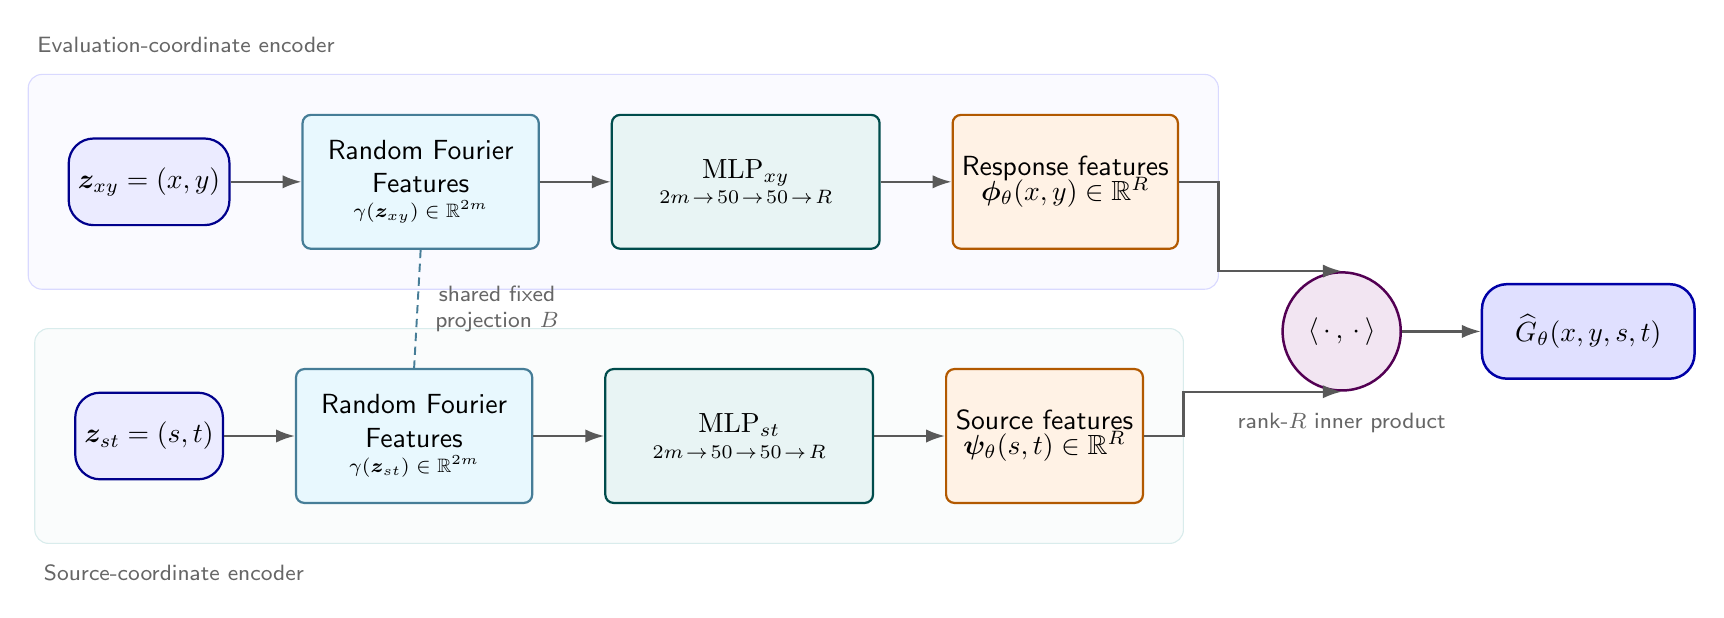
\begin{tikzpicture}[
    font=\sffamily,
    >={Latex[length=2.4mm,width=1.7mm]},
    flow/.style={->,draw=black!65,line width=0.8pt},
    input/.style={rounded corners=9pt,draw=blue!55!black,fill=blue!8,
      minimum width=16mm,minimum height=11mm,line width=0.8pt},
    rff/.style={rounded corners=3pt,draw=cyan!55!black,fill=cyan!9,
      minimum width=30mm,minimum height=17mm,align=center,line width=0.8pt},
    mlp/.style={rounded corners=3pt,draw=teal!60!black,fill=teal!9,
      minimum width=34mm,minimum height=17mm,align=center,line width=0.8pt},
    feature/.style={rounded corners=3pt,draw=orange!70!black,fill=orange!10,
      minimum width=25mm,minimum height=17mm,align=center,line width=0.8pt},
    merge/.style={circle,draw=violet!65!black,fill=violet!10,
      minimum size=15mm,line width=0.9pt,align=center},
    output/.style={rounded corners=9pt,draw=blue!65!black,fill=blue!12,
      minimum width=27mm,minimum height=12mm,line width=0.9pt},
    note/.style={font=\footnotesize\sffamily,text=black!60,align=center}
  ]
    \node[input] (xy) {$\bm z_{xy}=(x,y)$};
    \node[rff,right=9mm of xy] (rffxy) {Random Fourier\\Features\\[-1mm]\scriptsize $\gamma(\bm z_{xy})\in\R^{2m}$};
    \node[mlp,right=9mm of rffxy] (mlpxy) {$\mathrm{MLP}_{xy}$\\[-1mm]\scriptsize $2m\!\to\!50\!\to\!50\!\to\!R$};
    \node[feature,right=9mm of mlpxy] (phi) {Response features\\[-1mm]$\bm\phi_\theta(x,y)\in\R^R$};

    \node[input,below=21mm of xy] (st) {$\bm z_{st}=(s,t)$};
    \node[rff,right=9mm of st] (rffst) {Random Fourier\\Features\\[-1mm]\scriptsize $\gamma(\bm z_{st})\in\R^{2m}$};
    \node[mlp,right=9mm of rffst] (mlpst) {$\mathrm{MLP}_{st}$\\[-1mm]\scriptsize $2m\!\to\!50\!\to\!50\!\to\!R$};
    \node[feature,right=9mm of mlpst] (psi) {Source features\\[-1mm]$\bm\psi_\theta(s,t)\in\R^R$};

    \node[merge,right=13mm of phi,yshift=-19mm] (dot) {$\langle\,\cdot\,,\,\cdot\,\rangle$};
    \node[output,right=10mm of dot] (g) {$\widehat G_\theta(x,y,s,t)$};

    \draw[flow] (xy) -- (rffxy);
    \draw[flow] (rffxy) -- (mlpxy);
    \draw[flow] (mlpxy) -- (phi);
    \draw[flow] (st) -- (rffst);
    \draw[flow] (rffst) -- (mlpst);
    \draw[flow] (mlpst) -- (psi);
    \draw[flow] (phi.east) -- ++(5mm,0) |- (dot.north);
    \draw[flow] (psi.east) -- ++(5mm,0) |- (dot.south);
    \draw[flow] (dot) -- (g);
    \node[note,below=1.5mm of dot] {rank-$R$ inner product};

    \draw[densely dashed,draw=cyan!55!black,line width=0.7pt]
      (rffxy.south) -- node[note,right,xshift=1mm] {shared fixed\\projection $B$} (rffst.north);

    \begin{scope}[on background layer]
      \node[fit=(xy)(rffxy)(mlpxy)(phi),rounded corners=5pt,
        fill=blue!2,draw=blue!15,inner sep=5mm] (upperlane) {};
      \node[fit=(st)(rffst)(mlpst)(psi),rounded corners=5pt,
        fill=teal!2,draw=teal!15,inner sep=5mm] (lowerlane) {};
    \end{scope}
    \node[note,above=1.5mm of upperlane.north west,anchor=south west]
      {Evaluation-coordinate encoder};
    \node[note,below=1.5mm of lowerlane.south west,anchor=north west]
      {Source-coordinate encoder};
  \end{tikzpicture}%
  }
  \caption{Factorized Plan A architecture. Evaluation and source coordinates pass through a shared fixed random Fourier feature map and two independently trained MLPs. The inner product of their rank-$R$ feature vectors produces the Green's-kernel value $\widehat G_\theta(x,y,s,t)$.}
  \label{fig:architecture}
\end{figure}

\subsection{Plan B: Direct Four-Dimensional Kernel}

Plan B represents the Green's kernel with a single network applied directly to the complete coordinate tuple. Let $\bm z_4=(x,y,s,t)\in\R^4$ and let $\gamma_{4D}:\R^4\rightarrow\R^{2m}$ denote its random Fourier feature map. The predicted kernel is
\begin{equation}
  \widehat G^{\mathrm{4D}}_{\theta}(x,y,s,t)
  =\operatorname{MLP}_{4D}\!\left(\gamma_{4D}(\bm z_4)\right).
  \label{eq:planB}
\end{equation}
The MLP has two hidden layers of width 50 with GELU activations and a scalar output, corresponding to the layer dimensions $100\rightarrow50\rightarrow50\rightarrow1$.
 With 100 Fourier frequencies, Plan B contains 12,651 trainable parameters. Unlike Plan A, this representation does not impose a separable low-rank structure and can, in principle,
  learn general interactions among all four coordinates. Its principal disadvantage is that the network must be evaluated independently at every four-dimensional grid tuple.

\begin{figure}[H]
  \centering
  \resizebox{0.94\linewidth}{!}{%
  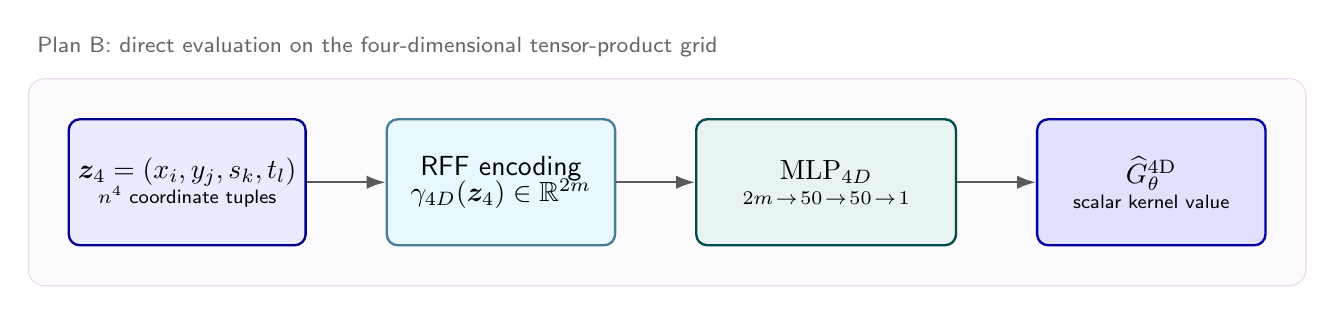
\begin{tikzpicture}[
    font=\sffamily,
    >={Latex[length=2.4mm,width=1.7mm]},
    flow/.style={->,draw=black!65,line width=0.8pt},
    stage/.style={rounded corners=4pt,minimum height=16mm,align=center,line width=0.85pt},
    note/.style={font=\footnotesize\sffamily,text=black!60,align=center}
  ]
    \node[stage,draw=blue!55!black,fill=blue!8,minimum width=30mm] (coords)
      {$\bm z_4=(x_i,y_j,s_k,t_l)$\\[-1mm]
       \scriptsize $n^4$ coordinate tuples};
    \node[stage,right=10mm of coords,draw=cyan!55!black,fill=cyan!9,
      minimum width=29mm] (rff)
      {RFF encoding\\[-1mm]
       $\gamma_{4D}(\bm z_4)\in\R^{2m}$};
    \node[stage,right=10mm of rff,draw=teal!60!black,fill=teal!9,
      minimum width=33mm] (mlp)
      {$\operatorname{MLP}_{4D}$\\[-1mm]
       \scriptsize $2m\!\to\!50\!\to\!50\!\to\!1$};
    \node[stage,right=10mm of mlp,draw=blue!65!black,fill=blue!12,
      minimum width=29mm] (out)
      {$\widehat G^{\mathrm{4D}}_\theta$\\[-1mm]
       \scriptsize scalar kernel value};

    \draw[flow] (coords) -- (rff);
    \draw[flow] (rff) -- (mlp);
    \draw[flow] (mlp) -- (out);

    \begin{scope}[on background layer]
      \node[fit=(coords)(rff)(mlp)(out),rounded corners=6pt,
        fill=violet!2,draw=violet!15,inner sep=5mm] (frame) {};
    \end{scope}
    \node[note,above=1.5mm of frame.north west,anchor=south west]
      {Plan B: direct evaluation on the four-dimensional tensor-product grid};
  \end{tikzpicture}%
  }
  \caption{Direct Plan B architecture. Each coordinate tuple $(x_i,y_j,s_k,t_l)$ is encoded jointly and passed through one four-input MLP to produce a scalar Green's-kernel value. The same network is evaluated independently at all $n^4$ tuples.}
  \label{fig:planB-architecture}
\end{figure}

Although Plan A contains more trainable parameters than Plan B, its MLPs are evaluated at substantially fewer coordinate locations. On an $n\times n$ spatial grid, the two Plan A encoders process $2n^2$ coordinate pairs, whereas Plan B processes all $n^4$ tuples $(x_i,y_j,s_k,t_l)$. For the $n=23$ grid used in this work, these counts are 1,058 and 279,841, respectively; Plan A therefore requires approximately 264.5 times fewer coordinate-wise MLP evaluations. This reduction concerns the neural-network evaluation rather than the complete algorithm: both implementations still materialize the $n^4$ Green's tensor for quadrature, so their final kernel-storage cost remains $O(n^4)$. Avoiding this materialization for Plan A is discussed in \cref{sec:limitations}.

\section{Physics-Informed Training}

For a mini-batch of $M$ random fields, the predicted solution for sample $q$ is computed from \cref{eq:quadrature}. Define the reconstruction residual and PDE residual by
\begin{align}
  R_{1}^{(q)} &= \widehat{U}^{(q)}-U^{(q)},\\
  R_{2}^{(q)} &= \Delta_h\widehat{U}^{(q)}-F^{(q)}.
\end{align}
The loss function is MSE loss:
\begin{equation}
  \mathcal{L}(\theta)=\frac{1}{Mn^2}
  \sum_{q=1}^{M}\sum_{i,j}
  \left[
  \left(R_{1,ij}^{(q)}\right)^2
  +\lambda\left(R_{2,ij}^{(q)}\right)^2
  \right].
  \label{eq:loss}
\end{equation}
The PDE weight is $\lambda=10^{-4}$. Optimization uses AdamW with initial learning rate $10^{-3}$, weight decay $10^{-6}$, and cosine annealing to $10^{-5}$ over 10,001 iterations. The batch size is 16, while a separately generated sample is used for validation. The best state according to the training loss is retained.

\begin{table}[H]
  \centering
  \caption{Configuration used to train Plan A and Plan B.}
  \label{tab:settings}
  \begin{tabular}{@{}ll@{}}
    \toprule
    Setting & Value \\
    \midrule
    Domain & $[-1,1]^2$ \\
    GLL polynomial order & $N=22$ ($23\times23$ grid) \\
    Fourier modes in training fields & $K=4$ \\
    Spectral decay exponent & $\alpha=2$ \\
    Random Fourier features & m=100 \\
    Hidden widths & 50, 50 \\
    Activation & GELU \\
    Kernel rank & $R=50$ \\
    Trainable parameters & Plan A: 30,300; Plan B: 12,651 \\
    Batch size & 16 \\
    Optimizer & AdamW \\
    Iterations & 10,001 \\
    PDE-loss weight & $10^{-4}$ \\
    Data refresh interval & 100 iterations \\
    \bottomrule
  \end{tabular}
\end{table}

\section{Experimental Design and Results}

\subsection{Compared architectures}

The two parameterizations defined in \cref{eq:lowrank,eq:planB} are trained and evaluated under a common experimental protocol. Plan A is treated as the proposed structured model and Plan B as the direct baseline. Both plans use the same GLL grid, Fourier feature scale, optimizer, number of updates, training-field generator, and loss weight. Their hidden-layer widths are also matched, while their output structures and parameter counts follow from the respective low-rank and direct kernel representations.

\begin{table}[H]
  \centering
  \caption{Neural-network evaluation cost and measured training time. The timing comparison uses the same training configuration for both plans.}
  \label{tab:training-cost}
  \begin{tabular}{@{}lrrrr@{}}
    \toprule
    Method & Parameters & MLP inputs/sample & Training time & Relative time \\
    \midrule
    Plan A: factorized 2D & 30,300 & 1,058 & 5 min 37 s & $1.0\times$ \\
    Plan B: direct 4D     & 12,651 & 279,841 & 233 min 16 s & $41.5\times$ \\
    \bottomrule
  \end{tabular}
\end{table}

Despite having more trainable parameters, Plan A is substantially faster than Plan B. Its training time is 5 min 37 s, compared with 233 min 16 s for Plan B, corresponding to an approximately 41.5-fold speedup. The main source of this difference is the reduction from $n^4$ direct four-dimensional MLP evaluations to two sets of $n^2$ encoder evaluations described in \cref{fig:architecture}. The measured speedup is smaller than the 264.5-fold ratio of MLP input locations because both plans still construct the full $n^4$ Green's tensor and perform the same numerical quadrature.

\subsection{Test functions}

Two zero-Dirichlet problems are used to probe different forms of generalization. Neither test function is included in the training mini-batches.

\paragraph{Test 1: unseen mixed-frequency field.}
The first test combines three Fourier modes, including frequencies above the training cutoff $K=4$:
\begin{align}
  u_1(x,y)={}&
  \sin\!\left(\frac{\pi(x+1)}{2}\right)
  \sin\!\left(\frac{2\pi(y+1)}{2}\right) \notag\\
  &+0.35\sin\!\left(\frac{5\pi(x+1)}{2}\right)
  \sin\!\left(\frac{3\pi(y+1)}{2}\right) \notag\\
  &-0.20\sin\!\left(\frac{7\pi(x+1)}{2}\right)
  \sin\!\left(\frac{\pi(y+1)}{2}\right),
  \label{eq:test1u}\\
  f_1(x,y)={}&
  -\frac{5\pi^2}{4}u_{1,2}(x,y)
  -0.35\frac{34\pi^2}{4}u_{5,3}(x,y)
  +0.20\frac{50\pi^2}{4}u_{7,1}(x,y),
  \label{eq:test1f}
\end{align}
where $u_{p,q}(x,y)=\sin(p\pi(x+1)/2)\sin(q\pi(y+1)/2)$. This problem tests whether the learned operator extrapolates beyond the frequencies used to generate the training fields.

\paragraph{Test 2: non-Fourier polynomial field.}
The second solution is
\begin{equation}
  u_2(x,y)=(1-x^2)(1-y^2)\left(1+\frac{x}{2}+\frac{y}{4}\right),
  \label{eq:test2u}
\end{equation}
with analytic forcing
\begin{align}
  f_2(x,y)={}&(1-y^2)\left[-2c(x,y)-2x\right]
  +(1-x^2)\left[-2c(x,y)-y\right],\label{eq:test2f}\\
  c(x,y)={}&1+\frac{x}{2}+\frac{y}{4}.
\end{align}
This field is smooth and satisfies the boundary condition exactly, but it is not itself a finite sine-mode sample. It therefore measures generalization outside the explicit data-generation family.

For a consistent comparison across both tests, we report the relative discrete $L^2$ error
\begin{equation}
  E_{2,\mathrm{rel}}=
  \frac{\norm{\widehat{U}-U}_2}{\norm{U}_2}.
  \label{eq:relativeL2}
\end{equation}
and the maximum nodal error $E_\infty=\max_{i,j}|\widehat{U}_{ij}-U_{ij}|$. The analytical forcing functions in \cref{eq:test1f,eq:test2f} are used in the Green's-function quadrature.

\begin{table}[H]
  \centering
  \caption{Generalization results for the two test functions.}
  \label{tab:newtests}
  \begin{tabular}{@{}llcc@{}}
    \toprule
    Test & Method & $E_\infty$ & $E_{2,\mathrm{rel}}$ \\
    \midrule
    Mixed frequency & Plan A: factorized 2D & $2.72\times10^{-2}$ & $6.53\times10^{-1}$ \\
                    & Plan B: direct 4D     & $1.96\times10^{-2}$ & $5.73\times10^{-1}$ \\
    Polynomial      & Plan A: factorized 2D & $2.72\times10^{-2}$ & $4.79\times10^{-2}$ \\
                    & Plan B: direct 4D     & $1.96\times10^{-2}$ & $4.70\times10^{-2}$ \\
    \bottomrule
  \end{tabular}
\end{table}

\subsection{Training behavior}

\Cref{fig:loss} shows the training and validation histories. Both plans reduce the training objective rapidly during the initial iterations and reach training losses below $10^{-4}$. The periodic sawtooth pattern follows the replacement of the random-function mini-batch every 100 iterations. Plan A's validation loss settles at a few times $10^{-3}$, whereas Plan B reaches the $10^{-4}$ range. The gap between training and validation is consistent with the greater difficulty of learning an operator that transfers across randomly generated functions.

\begin{figure}[H]
  \centering
  \begin{subfigure}[t]{0.48\linewidth}
    \centering
    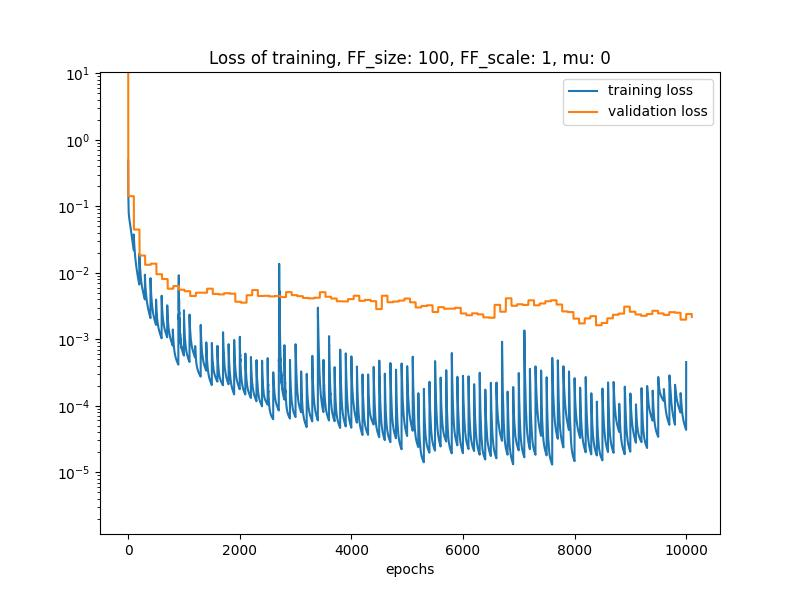
\includegraphics[width=\linewidth]{figures/loss_planA.jpg}
    \caption{Plan A: factorized 2D model.}
  \end{subfigure}
  \hfill
  \begin{subfigure}[t]{0.48\linewidth}
    \centering
    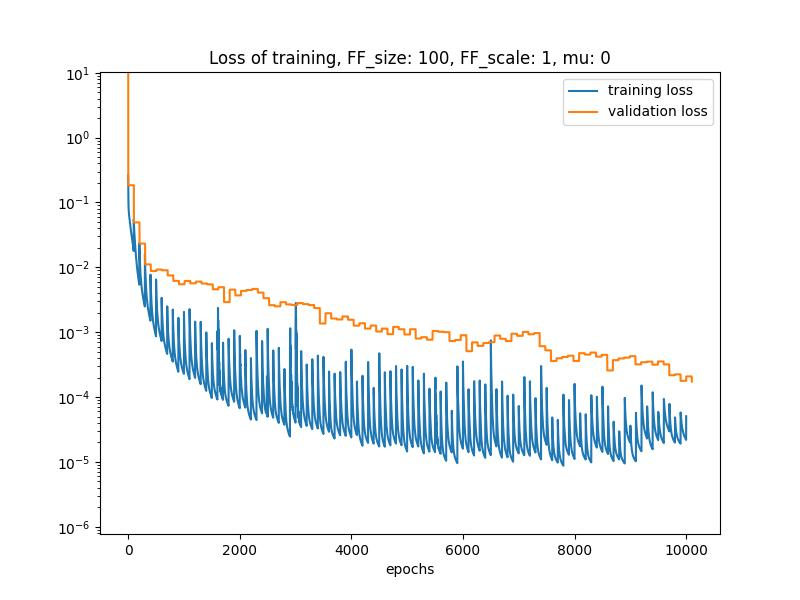
\includegraphics[width=\linewidth]{figures/loss_planB.jpg}
    \caption{Plan B: direct 4D model.}
  \end{subfigure}
  \caption{Training and validation loss over 10,001 optimization steps.}
  \label{fig:loss}
\end{figure}

\subsection{Mixed-frequency generalization}

The mixed-frequency test is substantially harder than the training distribution because it contains the $(5,3)$ and $(7,1)$ modes, while training is restricted to $k_x,k_y\leq4$. Plan A obtains $E_\infty=2.72\times10^{-2}$ and $E_{2,\mathrm{rel}}=6.53\times10^{-1}$, whereas Plan B obtains $E_\infty=1.96\times10^{-2}$ and $E_{2,\mathrm{rel}}=5.73\times10^{-1}$. Thus, Plan B reduces the relative error by approximately $12.3\%$ with respect to Plan A, but both relative errors remain large. As shown in \cref{fig:multimode}, both networks reproduce the broad sign-changing structure but distort the amplitudes and high-frequency details. This experiment indicates that neither architecture reliably extrapolates to spatial frequencies absent from the training ensemble.

\begin{figure}[H]
  \centering
  \begin{subfigure}[t]{0.49\linewidth}
    \centering
    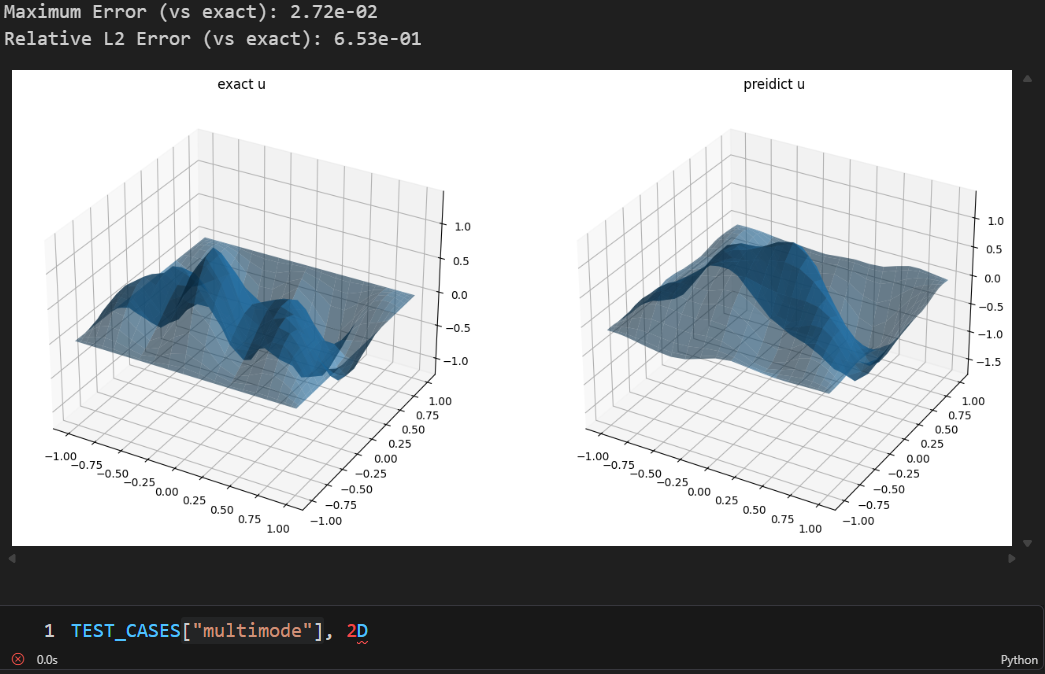
\includegraphics[width=\linewidth,trim=20 140 50 80,clip]{figures/multimode_planA.png}
    \caption{Plan A: $E_\infty=2.72\times10^{-2}$, $E_{2,\mathrm{rel}}=6.53\times10^{-1}$.}
  \end{subfigure}
  \hfill
  \begin{subfigure}[t]{0.49\linewidth}
    \centering
    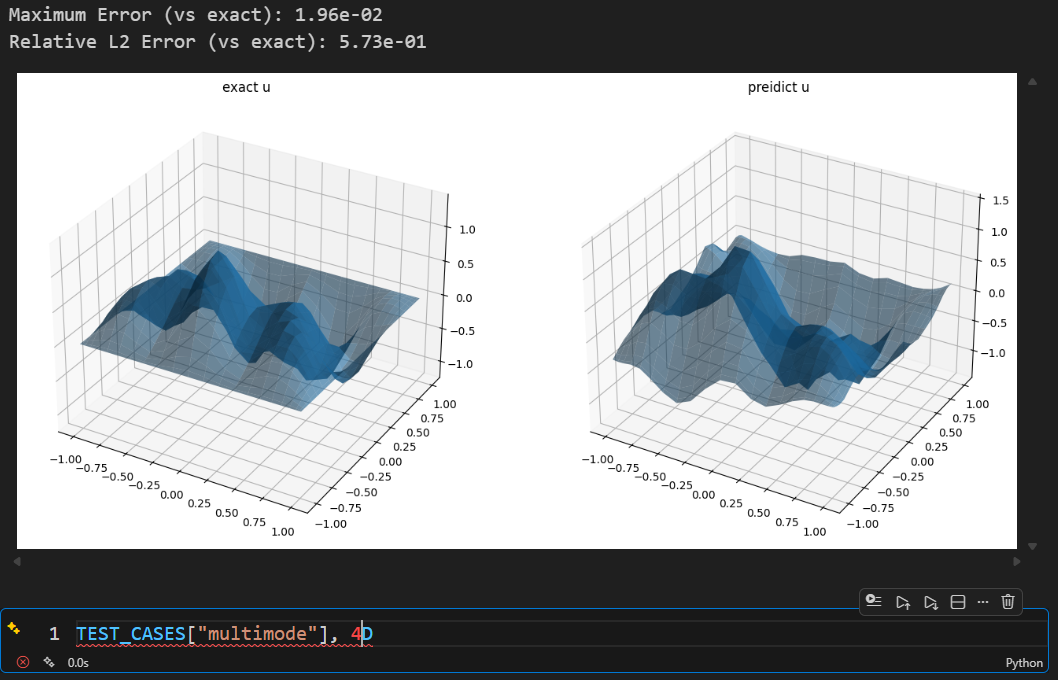
\includegraphics[width=\linewidth,trim=20 140 50 80,clip]{figures/multimode_planB.png}
    \caption{Plan B: $E_\infty=1.96\times10^{-2}$, $E_{2,\mathrm{rel}}=5.73\times10^{-1}$.}
  \end{subfigure}
  \caption{Exact (left panel within each subfigure) and predicted (right panel) mixed-frequency solutions.}
  \label{fig:multimode}
\end{figure}

\subsection{Polynomial generalization}

Both architectures generalize much more accurately to the smooth polynomial field. Plan A gives $E_{2,\mathrm{rel}}=4.79\times10^{-2}$ and $E_\infty=2.72\times10^{-2}$, while Plan B gives $E_{2,\mathrm{rel}}=4.70\times10^{-2}$ and $E_\infty=1.96\times10^{-2}$. The relative errors differ by less than one percentage point, showing nearly equivalent global accuracy. Plan B has the smaller maximum nodal error, but both predictions closely match the exact dome-shaped surface in \cref{fig:polynomial}. The result demonstrates that training on random sine fields can transfer to a smooth function outside the finite Fourier family when its spatial scale remains compatible with the training distribution.

\begin{figure}[H]
  \centering
  \begin{subfigure}[t]{0.49\linewidth}
    \centering
    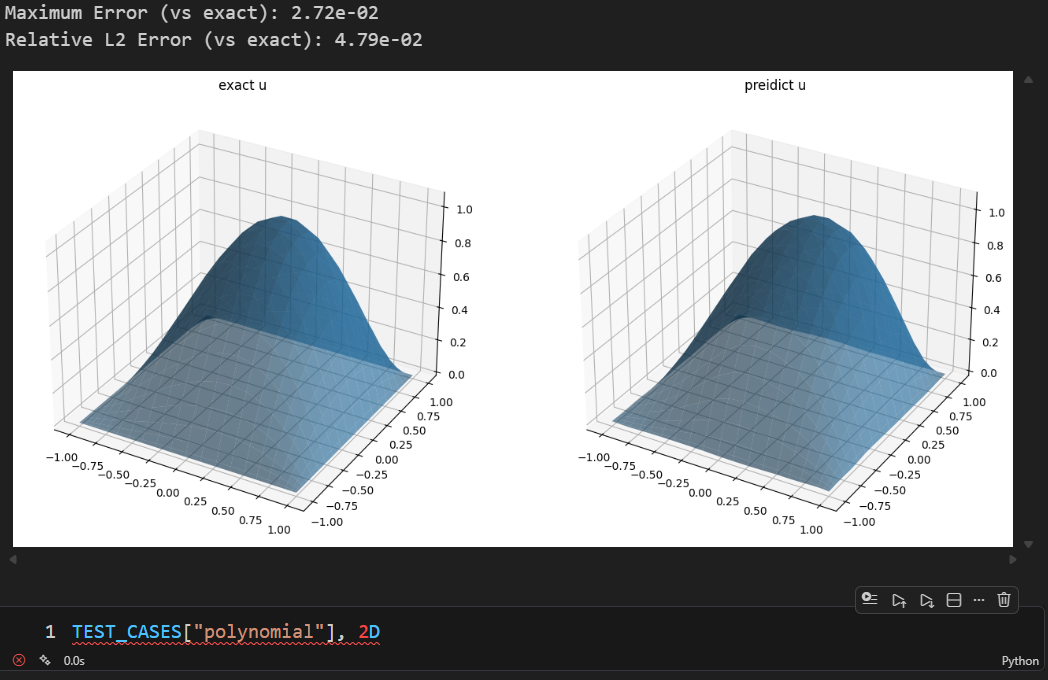
\includegraphics[width=\linewidth,trim=20 140 50 80,clip]{figures/polynomial_planA.png}
    \caption{Plan A: $E_\infty=2.72\times10^{-2}$, $E_{2,\mathrm{rel}}=4.79\times10^{-2}$.}
  \end{subfigure}
  \hfill
  \begin{subfigure}[t]{0.49\linewidth}
    \centering
    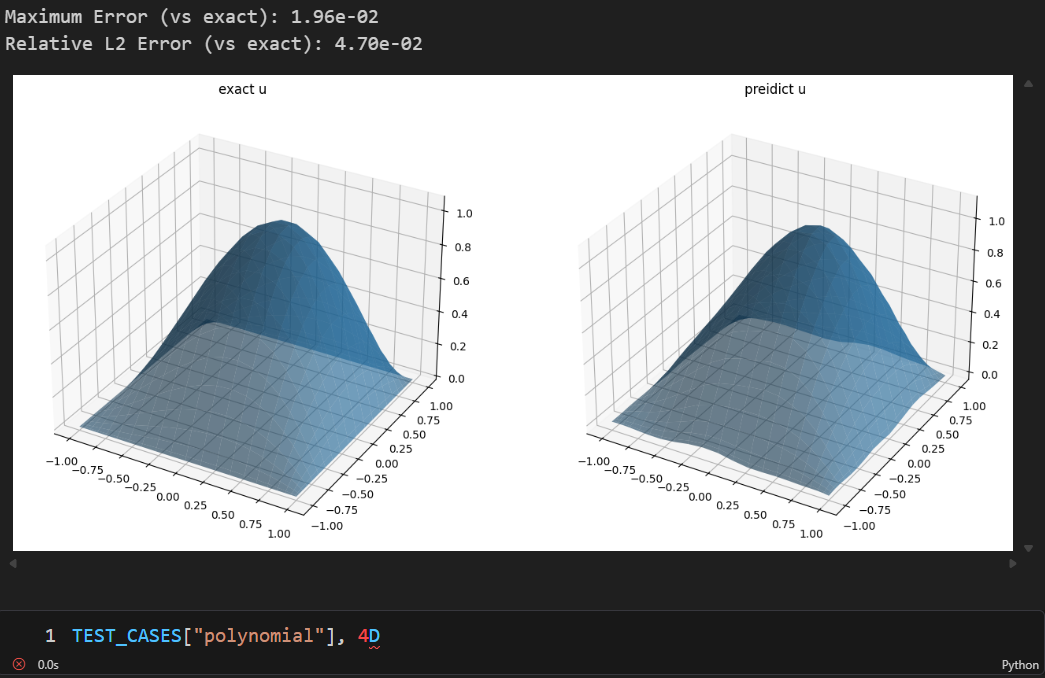
\includegraphics[width=\linewidth,trim=20 140 50 80,clip]{figures/polynomial_planB.png}
    \caption{Plan B: $E_\infty=1.96\times10^{-2}$, $E_{2,\mathrm{rel}}=4.70\times10^{-2}$.}
  \end{subfigure}
  \caption{Exact (left panel within each subfigure) and predicted (right panel) polynomial solutions.}
  \label{fig:polynomial}
\end{figure}

\section{Discussion}

The experiments demonstrate that the solution of a linear PDE can be reconstructed from a learned kernel rather than from a network specialized to one forcing term. Three aspects are particularly important.

First, the random Fourier generator provides exact and inexpensive training pairs. Spectral decay biases the samples toward smooth fields, and the sine basis enforces zero boundary values. The polynomial result shows that the learned mapping is not restricted to reproducing individual sine-series samples. In contrast, the mixed-frequency result reveals a clear spectral limitation: modes above the training cutoff produce relative errors exceeding $0.5$ for both plans. Extending the frequency content and smoothness range of the training ensemble is therefore more important than choosing between the two tested architectures for this case.

Second, the factorized kernel substantially reduces neural evaluation cost. The two encoders evaluate only $2n^2$ coordinate locations, after which an outer product constructs the kernel. This is attractive for increasing network depth or width, and the rank $R$ is an interpretable accuracy--cost parameter. Plan A closely matches Plan B on the polynomial test, although Plan B performs moderately better on the unseen high-frequency field. This suggests that the low-rank representation is adequate for smooth responses but should be tested over multiple ranks before drawing a general conclusion.

Third, the combined loss constrains both the integral reconstruction and the governing PDE. The reconstruction term anchors the action of the operator on sampled functions, while the residual term discourages outputs that violate the discrete Poisson equation. Because $\lambda=10^{-4}$ is small, the current balance emphasizes reconstruction. A systematic study of this parameter would be valuable.

\section{Limitations and Future Work}
\label{sec:limitations}

Several limitations should be addressed before claiming a general Green's-function solver:

\begin{itemize}[leftmargin=2em]
  \item \textbf{Boundary enforcement.} The solution samples satisfy homogeneous boundary conditions, but the neural kernel itself is not explicitly constrained to vanish on the appropriate boundary. A multiplicative boundary mask or a dedicated boundary loss could impose this property exactly or approximately.
  \item \textbf{Kernel identifiability.} Training only through $Gf\approx u$ constrains the action of the kernel on the sampled forcing subspace. It does not uniquely identify the full continuous Green's function outside that subspace. Direct constraints based on reciprocity, boundary values, or the adjoint Green's equation could reduce this ambiguity.
  \item \textbf{Materialization cost.} Although the encoders are evaluated on $O(n^2)$ inputs, the code constructs an $O(n^4)$ tensor. Using the factorization directly gives
  \begin{equation}
    \uhat(x_i,y_j)=\sum_{r=1}^{R}\phi_r(x_i,y_j)
    \left[\sum_{k,l}\psi_r(s_k,t_l)f_{kl}w_kw_l\right],
  \end{equation}
  which reduces storage and contraction cost to quantities scaling with $Rn^2$.
  \item \textbf{Validation breadth.} The tests cover a smooth polynomial and an unseen mixed-frequency field. Further studies should include localized sources, varying smoothness, multiple random seeds, and comparisons with spectral or finite-element reference solvers.
  \item \textbf{Continuous versus discrete forcing.} Comparing the analytical forcing with the grid-consistent choice $F_h=\Delta_hU$ would separate operator approximation error from spectral discretization error.
\end{itemize}

\section{Conclusion}

We developed a physics-informed, low-rank neural approximation of the Green's operator for the two-dimensional Poisson equation and compared it with a direct four-dimensional neural kernel. The method combines random Fourier training fields, GLL spectral discretization, random Fourier feature encodings, and a separable rank-50 representation. Both architectures reconstruct the smooth non-Fourier polynomial solution with relative $L^2$ error below $4.8\times10^{-2}$, demonstrating useful transfer beyond the explicit training family. Their errors rise to $6.53\times10^{-1}$ and $5.73\times10^{-1}$ on the mixed-frequency problem, identifying training-spectrum coverage as the principal limitation. Plan A therefore offers a promising structured representation for smooth operator learning, while broader spectral training, robust boundary enforcement, rank studies, and contraction without explicit four-dimensional kernel materialization remain necessary for a scalable and general neural PDE solver.

\footnotesize
\begin{thebibliography}{9}

\bibitem{raissi2019pinn}
M.~Raissi, P.~Perdikaris, and G.~E.~Karniadakis,
``Physics-informed neural networks: A deep learning framework for solving forward and inverse problems involving nonlinear partial differential equations,''
\emph{Journal of Computational Physics}, vol.~378, pp.~686--707, 2019.

\bibitem{lu2021deeponet}
L.~Lu, P.~Jin, G.~Pang, Z.~Zhang, and G.~E.~Karniadakis,
``Learning nonlinear operators via DeepONet based on the universal approximation theorem of operators,''
\emph{Nature Machine Intelligence}, vol.~3, pp.~218--229, 2021.

\bibitem{li2021fno}
Z.~Li, N.~Kovachki, K.~Azizzadenesheli, B.~Liu, K.~Bhattacharya, A.~Stuart, and A.~Anandkumar,
``Fourier neural operator for parametric partial differential equations,''
in \emph{Proceedings of the International Conference on Learning Representations}, 2021.

\bibitem{tancik2020fourier}
M.~Tancik, P.~Srinivasan, B.~Mildenhall, S.~Fridovich-Keil, N.~Raghavan, U.~Singhal, R.~Ramamoorthi, J.~Barron, and R.~Ng,
``Fourier features let networks learn high frequency functions in low dimensional domains,''
in \emph{Advances in Neural Information Processing Systems}, vol.~33, pp.~7537--7547, 2020.

\bibitem{karniadakis2021physics}
G.~E.~Karniadakis, I.~G.~Kevrekidis, L.~Lu, P.~Perdikaris, S.~Wang, and L.~Yang,
``Physics-informed machine learning,''
\emph{Nature Reviews Physics}, vol.~3, pp.~422--440, 2021.

\end{thebibliography}

\end{document}
